\documentclass{article}
%packages
\usepackage{graphicx}
\usepackage[utf8]{inputenc}
\usepackage[T1]{fontenc}
\usepackage[frenchb]{babel}
\usepackage[a4paper]{geometry}
\usepackage{minted}

\begin{document}
%title
\begin{titlepage}
	\vspace{-20px}
	\begin{tabular}{l}
		\textsc{Blin} S\'ebastien\\
		\textsc{Collin} Pierre-Henri
	\end{tabular}
	\hfill \vspace{10px}
\includegraphics[scale=0.1]{esir.png}\\
	\vfill
	\begin{center}
		\Huge{\'Ecole sup\'erieure d'ing\'enieurs de Rennes}\\
		\vspace{1cm}
		\LARGE{1\`ere Ann\'ee}\\
		\large{Parcours Informatique}\\
		\vspace{0.5cm}\hrule\vspace{0.5cm}
		\LARGE{\textbf{Algorithmie et complexité}}\\
		\Large{Compte-Rendu TP3}
		\vspace{0.5cm}\hrule
		\vfill
		\vfill
	\end{center}
	\begin{flushleft}
		\Large{Sous l'encadrement de~:}\\
		\vspace{0.2cm}
		\large{{Ridoux} Olivier}\\
		\large{{Maurel} Pierre}
	\end{flushleft}
	\vfill
\end{titlepage}

L'objectif de ce TP 3 est de créer un programme qui calcule le ROBDD associé à une expression booléenne et de comparer ses performances à celles d'un arbre de décision (arbre de Shannon).
\section{Prise en main des expressions booléennes}
\subsection{Objectif}
Le but de cette partie est de se familiariser avec les classes proposées pour créer des expressions booléennes (Et, Ou, Non, et Implique) et apprendre à les manipuler.
\subsection{Programmation des méthodes dans les classes Atome et Equiv}
\subsubsection{La classe Equiv}
\begin{minted}{java}
public boolean evalue() throws RuntimeException {
	return e1.evalue() == e2.evalue();
}

public Set<String> atomes() {
	Set<String> s = new HashSet<String>();
	s.addAll(e1.atomes());
	s.addAll(e2.atomes());
	return s;
}

public Expression remplace(String s, boolean b) {
	return new Equiv(e1.remplace(s, b),e2.remplace(s, b));
}
\end{minted}
\subsubsection{La classe Atome}
\begin{minted}{java}
public Set<String> atomes() {
	Set<String> s = new HashSet<String>();
	s.add(name);
	return s;
}

public Expression remplace(String s, boolean b) {
	if (name.equals(s))
		return new Constante(b);
	else
		return this;
}

public Expression simplifier(){
	return this;
}
\end{minted}
\subsection{Résultats}
Afin de tester les différentes fonctions de la classe Expression, nous avons créé l'expression booléenne suivante : \\
\begin{verbatim}
Expression ex2 = new Et(
                      new Equiv(new Atome("x1"),new Atome("y1")), 
                      new Equiv(new Atome("x2"),new Atome("y2"))
                      );
\end{verbatim}
$x1\Longleftrightarrow y1\wedge x2\Longleftrightarrow y2$\\
On peut remplacer les atomes par des valeurs booléennes puis, évaluer l'expression :
\begin{minted}{java}
ex2 = ex2.remplace("x1",true);
ex2 = ex2.remplace("y1",true);
ex2 = ex2.remplace("x2",false);
ex2 = ex2.remplace("y2",false);
System.out.println(ex2.evalue());
\end{minted}
L'évaluation de cette expression nous renvoie true.\\
Ensuite, on créé un ordre des atomes :
\begin{minted}{java}
List<String> ordre_atomes = new LinkedList<String>();
ordre_atomes.add("x1");
ordre_atomes.add("y1");
ordre_atomes.add("x2");
ordre_atomes.add("y2");
\end{minted}
Affichage de l'arbre pour l'ordre suivant (x1 > y1 > x2 > y2) : \\\\
Arbre de ex2 : 
\begin{verbatim}
x1
|->y1
|   |->x2
|   |   |->y2
|   |   |   |->1
|   |   |   |->0
|   |   |->y2
|   |   |   |->0
|   |   |   |->1
|   |->x2
|   |   |->y2
|   |   |   |->0
|   |   |   |->0
|   |   |->y2
|   |   |   |->0
|   |   |   |->0
|->y1
|   |->x2
|   |   |->y2
|   |   |   |->0
|   |   |   |->0
|   |   |->y2
|   |   |   |->0
|   |   |   |->0
|   |->x2
|   |   |->y2
|   |   |   |->1
|   |   |   |->0
|   |   |->y2
|   |   |   |->0
|   |   |   |->1
\end{verbatim}
Affichage de l'arbre pour le deuxième ordre vu en TD (x1 > x2 > y1 > y2) : \\\\
Arbre de ex2 : 
\begin{verbatim}
x1
|->x2
|   |->y1
|   |   |->y2
|   |   |   |->1
|   |   |   |->0
|   |   |->y2
|   |   |   |->0
|   |   |   |->0
|   |->y1
|   |   |->y2
|   |   |   |->0
|   |   |   |->1
|   |   |->y2
|   |   |   |->0
|   |   |   |->0
|->x2
|   |->y1
|   |   |->y2
|   |   |   |->0
|   |   |   |->0
|   |   |->y2
|   |   |   |->1
|   |   |   |->0
|   |->y1
|   |   |->y2
|   |   |   |->0
|   |   |   |->0
|   |   |->y2
|   |   |   |->0
|   |   |   |->1
\end{verbatim}
On constate que les arbres obtenus correspondent bien à ceux trouvés en TD.
\subsection{Conclusion}
Nous avons donc vu dans cette partie qu'il est possible de créer des expressions booléennes, de remplacer des atomes, d'évaluer des expressions et d'afficher les arbres de Shannon correspondants. 
\section{Construction du ROBDD}
\subsection{Objectif}
Ici, nous allons voir comment construire le ROBDD d'une expression booléenne.
\subsection{Programmation des méthodes}
\subsubsection{Les fonctions estVrai() et estFaux()}
\begin{minted}{java}
public boolean estVrai(){
	return (this.atomes().equals(new HashSet<String>())) && this.evalue();
}

public boolean estFaux(){
	return (this.atomes().equals(new HashSet<String>())) && !this.evalue();
}
\end{minted}
\subsubsection{La fonction obtenirROBDDIndex}
\begin{minted}{java}
public int obtenirROBDDIndex(String nom, int fg, int fd) {
	Iterator<Noeud_ROBDD> it = R.iterator();
	while(it.hasNext())
	{
		Noeud_ROBDD n = it.next();
		if(n.getNom().equals(nom) && n.getIdFilsGauche() == fg 
		&& n.getIdFilsDroit() == fd)
			return n.getId();
	}
	return -1;
}
\end{minted}
\subsubsection{La fonction construireROBDD}
\begin{minted}{java}
private int construireROBDD(ROBDD G, List<String> atomes_ordonnes){
	List<String> atomes_ordonnes_copie = new LinkedList(atomes_ordonnes);
	Expression e = simplifier();
	if(e.estFaux()) return 0;
	if(e.estVrai()) return 1;
	
	String p = atomes_ordonnes_copie.remove(0);
	Expression exp = e.remplace(p, false);
	Expression exn = e.remplace(p, true);
	
	int n1 = exp.construireROBDD(G, atomes_ordonnes_copie);
	int n2 = exn.construireROBDD(G, atomes_ordonnes_copie);
	
	if(n1==n2)
		return n1;
	if(G.obtenirROBDDIndex(p, n1, n2) != -1)
		return G.obtenirROBDDIndex(p, n1, n2);
	else
	{
		Noeud_ROBDD n = new Noeud_ROBDD(p,n1,n2);
		G.ajouter(n);
		return n.getId();
	}
}
\end{minted}

Nous avons vérifié le bon fonctionnement de la fonction sur l'expression de l'exercice 2.\\
On obtient le résultat suivant : [2:bdd(x2,1,0), 3:bdd(x2,0,1), 4:bdd(y2,2,3), 5:bdd(x1,4,6:bdd(x1,0,4), 7:bdd(y1,5,6)].\\
On a également vérifié le résultat pour l'expression de l'exercice 10 du TD où on obtient : [2:bdd(z,0,1), 3:bdd(y,1,2), 4:bdd(y,0,1), 5:bdd(x,3,4)].\\
\subsubsection{La fonction trouve\_sat}
\begin{minted}{java}
public String trouve_sat()
{
	String ret = "";
	Iterator<Noeud_ROBDD> it = R.iterator();
	int toSearch = 1;
	while(it.hasNext())
	{
		Noeud_ROBDD n = it.next();
		if(n.getIdFilsDroit() == toSearch)
		{
			toSearch = n.getId();
			ret += n.getNom() + ".";
		}
		if(n.getIdFilsGauche() == toSearch)
			toSearch = n.getId();
	}
	
	if(toSearch == 1)
		return "Non SAT";
	else
		return ret;
}
\end{minted}
Nous avons testé cette fonction sur l'expression créée à l'exercice 2.
On obtient le résultat suivant : non x1, non y1, non x2, non y2
\subsection{Conclusion}
On a donc créé une fonction qui permet d'obtenir le ROBDD d'une fonction boléenne en implémentant l'algorithme récursif vu en TD. Pour cela, nous avons programmé des fonctions auxiliaires : estVrai(), estFaux() et obtenirROBDDIndex(). De plus, nous avons créé une fonction qui permet de parcourir un ROBDD et dire s'il est satisfaisable ou non.
\section{Problème des N reines}
\subsection{Objectif}
Dans la seconde partie de ce TP, nous devions utiliser les ROBDD pour pouvoir résoudre un problème. Le problème consiste à trouver une combinaison de cases où placer N dames sur un plateau de taille NxN pour ne pas qu'elles puissent se menacer mutuellement. Donc qu'il y en ait une par colonne, une par ligne, et pas 2 sur la même diagonale.\\
La solution consiste donc à modéliser une équation booléenne modélisant les conditions en prenant chaque case comme une variable.
\subsection{Moyens mis en \oe uvre}
L'expression finale est un ET logique entre 3 sous équations, puisque nous souhaitons avoir une dame par ligne ET une dame par colonne ET au maximum une dame par diagonale.\\
La première sous-équation décrit le fait qu'il y ait une dame par ligne.
\begin{minted}{java}
for(int i = 0; i < n; ++i)
{
	Expression temp2 = new Constante(false);
	for(int k = 0; k < n; ++k)
	{
		Expression temp = new Constante(true);
		for(int j = 0; j < n; ++j)
		{
			if(j != k)
				temp = new Et(new Non(new Atome("x"+ i + j)), temp);
			else
				temp = new Et(new Atome("x"+ i + j), temp);
		}
		temp2 = new Ou(temp2, temp);
	}
	expDame = new Et(expDame, temp2);
}
\end{minted}
Ce qui peut se traduire par $\vee_{(1 \geq i \geq N, 1 \geq j \geq N)}[x_{ij}\Rightarrow \wedge_{(1\geq l\geq N, l\neq j)}\neg x_{il}]$ avec au moins un $x_{ij}$ vrai. Même si dans notre code, nous le modélisons à l'aide de Et et de Ou logique.\\
Pour les colonnes, c'est à peut prêt la même méthode, il suffit d'échanger 2 boucles, on peut considérer le problème comme celui de résoudre une dame par ligne avec un plateau à 90 degrés.
\begin{minted}{java}
for(int j = 0; j < n; ++j)
{
	Expression temp2 = new Constante(false);
	for(int k = 0; k < n; ++k)
	{
		Expression temp = new Constante(true);
		for(int i = 0; i < n; ++i)
		{
			if(i != k)
				temp = new Et(new Non(new Atome("x"+ i + j)), temp);
			else
				temp = new Et(new Atome("x"+ i + j), temp);
		}
		temp2 = new Ou(temp2, temp);
	}
	expDame = new Et(expDame, temp2);
}
\end{minted}
Le traitement des diagonales est un peu différent. Ici, il faut considérer des droites et prendre seulement les cases dans le plateau. L'équation nous donne : $x_{ij}\Rightarrow \wedge_{(1\geq k\geq N, 1\geq j+k-i\geq N, k\neq i)}\neg x_{k,j+k-i}$ dans un sens, $x_{ij}\Rightarrow \wedge_{(1\geq k\geq N, 1\geq j+i-k\geq N, k\neq i)}\neg x_{k,j+i-k}$ pour l'autre sens.
\begin{minted}{java}
for(int i = 0; i < n; ++i)
{
	Expression temp2 = new Constante(false);
	for(int j = 0; j < n; ++j)
	{
		Expression temp = new Constante(true);
		for(int k = 0; k < n; ++k)
		{
			int v = j+k-i;
			int w = j+i-k;
			boolean find = false;
			if(i != k && v < n && v >= 0)
			{
				temp = new Et(new Non(new Atome("x" + k + v)), temp);
				find = true;
			}
			if(i!=k && w < n && w >= 0)
			{
				temp = new Et(new Non(new Atome("x" + k + w)), temp);
				find = true;
			}
			if(!find)
				temp = new Et(new Atome("x" + i + j), temp);
		}
		temp2 = new Ou(temp2, temp);
	}
	expDame = new Et(expDame, temp2);
}
\end{minted}
Ce qui nous permet de modéliser une équation booléenne représentant le fait de n'avoir qu'une dame par ligne, une par colonne et au maximum une par diagonale.\\
Enfin, pour la partie de l'affichage, il suffit de trouver une solution (première partie de la fonction) en parcourant le ROBDD de l'expression précédement créée et de stocker les cases où les dames sont présentes à true (via un tableau représentant linéairement le plateau). Puis on dessine avec la seconde partie de la fonction.
\begin{minted}{java}
//Affiche le tableau solution pour le probleme des dames
public void reines_affiche_sat(int n)
{
	//Le tableau contenant true pour les cases possedant une dame
	boolean[] solution = new boolean[n*n];
	Iterator<Noeud_ROBDD> it = R.iterator();
	int toSearch = 1;
	while(it.hasNext())
	{
		Noeud_ROBDD node = it.next();
		if(node.getIdFilsDroit() == toSearch)
		{
			toSearch = node.getId();
			try
			{
				//Pour savoir quelle variable correspond a quelle case
				Pattern p = Pattern.compile("x([0-9])([0-9])");
				Matcher m = p.matcher(node.getNom());
				m.matches();
				solution[Integer.parseInt(m.group(1))*n+
				Integer.parseInt(m.group(2))] = true;
			}
			catch (Exception e)
			{
			
			}
		}
		if(node.getIdFilsGauche() == toSearch)
			toSearch = node.getId();
	}
	
	/**Affichage**/
	for(int i = 0; i < n; ++i)
	{
		for(int j = 0; j < 3*n; ++j)
			System.out.print("_");
		System.out.print("\n");
		for(int j = 0; j < n; ++j)
			if(solution[i*n+j])
				System.out.print("|X|");
			else
				System.out.print("| |");
		System.out.print("\n");
	}
	for(int j = 0; j < 3*n; ++j)
		System.out.print("_");
	System.out.print("\n");
}
\end{minted}
\subsection{Résultats}
Pour un plateau de où N = :
\begin{itemize}
  \item 1 : x00
  \item 2, 3 : NON SAT
  \item 4 : x13.x01.x20.x32.
  \item 5 : x02.x21.x40.x14.x33.
  \item 6 : x02.x21.x40.x15.x34.x53.
  \item 7 : x01.x40.x32.x24.x63.x16.x55.
  \item 8 : x03.x41.x34.x76.x20.x62.x15.x57
\end{itemize}
\begin{figure}
	\begin{center}
		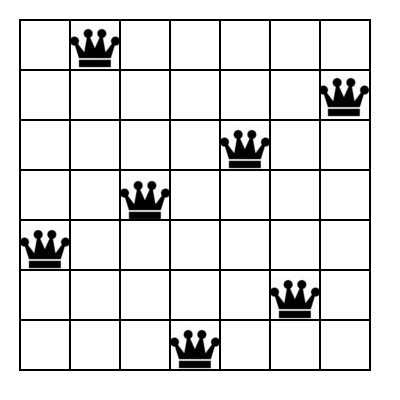
\includegraphics[scale=0.7]{sevenkingdom}\\
		Solution fournie par l'algorithme n=7 reines
	\end{center}
\end{figure}
\section{Conclusion}
Pour conclure, nous pouvons remarquer que choisir une représentation d'un problème de type SAT avec un ROBDD est une méthode qui fonctionne bien et dont le parcourt afin de trouver une solution est relativement rapide. Par contre, la taille du ROBDD peut très vite exploser. Par contre, la construction de notre ROBDD prend énormément de temps ce qui n'est pas normal. Nous n'avons donc pas pu comparer avec l'arbre de Shannon. (Même si logiquement l'arbre de Shannon a une taille plus grosse que le ROBDD)
\end{document}

